\section{Depth-Based Tiebreaking for A*}

\label{sec:depth}

% One useful notion which can be used to both understand and control the
% search in this situation is 
The \emph{depth} of a node is an integer value representing the distance
(number of steps) from the \emph{entrance} of the plateau on which the node is.
An \emph{entrance} of the plateau is the first state which entered the
plateau, along the path from the initial state. These notions are depicted
in \refig{fig:plateau-depiction}.

\begin{figure}[htbp]
 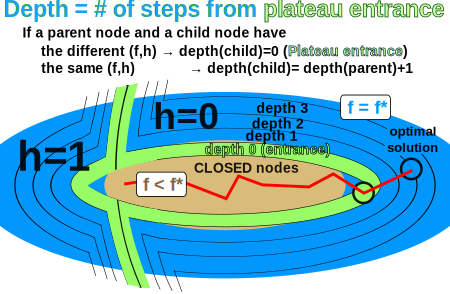
\includegraphics{img/astar/final-plateau4.png}
 \caption{The nodes in a platau are divided into several layers,
 and each layor have the corresponding depth.}
 \label{fig:plateau-depiction}
\end{figure}

The depth $d(s)$ of a
state $s$ is 0 when $s$ and the parent state $t$ has the different key
values for a sorting strategy, and $d(s)=d(t)+1$ when they have the same
key values: For example, in \astar with $h$-based tiebreaking, the key
values of a state are represented as a vector $[f,h]$, and they are same
when they are pairwise equivalent (i.e. $f(s) = f(t) \land h(s) =
h(t)$).  Having the same key values means that $s$ and $t$ are in the
same plateau. \todo{Figure}

% \textbf{XXX From SoCS draft}
% For such situations, they proposed a notion of \emph{depth} within the
% plateau, and an idea of diversifying the search over different depths
% within a plateau. 
% \textbf{XXX From SoCS draft}

% Given a node $n$,
% if its current parent $\parent{n}$ is from the other plateau, i.e.,
% $\parent{n}$ has a different $f$-value, or different $h$-value when the
% first tiebreaking is present, then $\depth{n} = 0$. Nodes with
% $\depth{n} = 0$ correspond to the \emph{entrance} of the plateau.  If $n$
% and $\parent{n}$ are in the same plateau i.e.\ share the same $f$ and $h$,
% $\depth{n}$ is defined as $\depth{\parent{n}} + 1$.  

Based on this simple notion of depth, we propose \emph{depth-based
tiebreaking} strategies, where the nodes are inserted into buckets
associated with depths, and upon expansion, search effort is distributed
among various depths. Notice that it does not ``sort'' the nodes
according to the depth, and instead ``diversify'' the node expansion
within the plateau. We mark such a diversification family of
tiebreaking strategies by enclosing it in brackets such as $[f,h,\brackets{d}]$.

In order to diversify the expansion among depths, we propose simply
iterating over the depth buckets. There is a counter $d_c$ initialized
to 0, which stores the depth which was selected in the last expansion.
In each expansion, it decrements the counter ($d_c\leftarrow d_c-1$) and
expands from the depth. When the counter reaches below 0, then the
counter is reset to the current largest depth in the plateau.
It is possible to adopt a
nondeterministic, randomized selection, as we have done in a conference
version of this paper, however we eliminate the possibility of the
results being affected by random seeds.
%  the buckets are chosen according to some policy.
% ``First depth'' (\fd), ``last depth'' (\ld), and ``random depth'' (\rd) 
% choose a bucket with the smallest depth,
% the largest depth, and a depth randomly selected at each expansion, respectively.

The traditional \lifo and \fifo tiebreaking strategy can be
considered as a ``sorting'' version of this depth-based tiebreaking.
\lifo strategy always select the most recently generated node
within $\plateau{f,h}$, and the behavior in the plateau is equivalent to depth-first search.
Thus, it results in always selecting the largest depth
buckets as depicted in \refig{fig:plateau-depiction-lifo}.
Similarly, the behavior of \fifo strategy 
in a plateau is equivalent to breadth-first search. Thus \fifo strategy
always selects the nodes with least depth (\refig{fig:plateau-depiction-fifo}).
Note that therefore $[f,h,\lifo]$ is equivalent to $[f,h,-d,\lifo]$ and
$[f,h,\fifo]$ is equivalent to $[f,h,d,\fifo]$.

\begin{figure}[htbp]
 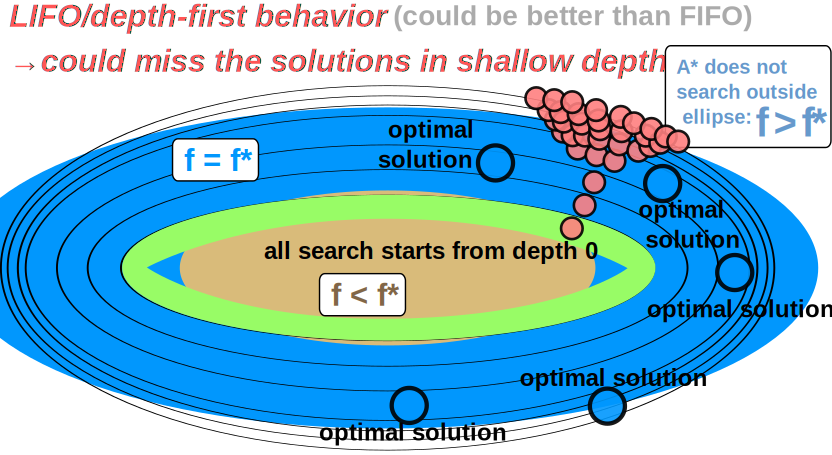
\includegraphics{img/astar/final-plateau6.png}
 \caption{\lifo tiebreaking strategy implies a depth-first behavior in a
 plateau, which could miss the solution concentrated near the entrance.}
 \label{fig:plateau-depiction-lifo}
\end{figure}

\begin{figure}[htbp]
 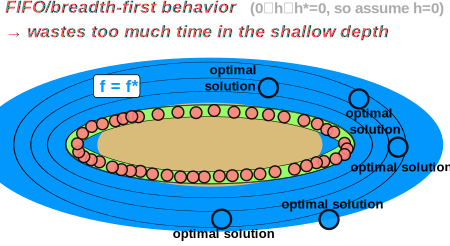
\includegraphics{img/astar/final-plateau5.png}
 \caption{\fifo tiebreaking strategy implies a breadth-first behavior in a
 plateau, which could fail to reach a solution in the deeper region
 within the time limit.}
 \label{fig:plateau-depiction-fifo}
\end{figure}


The problem in these traditional strategies is that we have no knowledge
on whether the goals are located near or far from the entrance. Remind
that when $f=f^*, h=h^*=0$, the goals in this plateau are optimal
regardless of the depth: Goals in the shallower region and the deeper
region both yield an optimal solution. However, until we find a
solution, we do not know how the goals are distributed among the
depths. In some problem instance the goals can be concentrated around
the entrance, and in another problem instance the goals can be
concentrated in some large depth $k$.

% \begin{figure}[htbp]
%  \includegraphics{img/astar/final-plateau4-2.png}
%  \label{fig:plateau-depiction-all-optimal}
% \end{figure}



The best-first search (\fifo), which naturally focus the search around
the entrance favoring the smaller depths, should perform better in the
former case, while it also severely degrade the performance when the
goals are located deep inside the plateau region because it searches the
shallower region exhaustively and takes too much time to reach the depth
where the goals exist.
Inversely, the depth-first search (\lifo), which greedily explores the
plateau region, may find a solution in the deeper region quickly but
could also miss the solution in the shallower region.

By an adversary argument, our depth-based \emph{diversification}
tiebreaking strategy, which diversify the search among various depths,
have no depth bias and eventually find a solution. It can be considered
similar to the random restarting strategy in tree search algorithms.

\begin{figure}[htbp]
 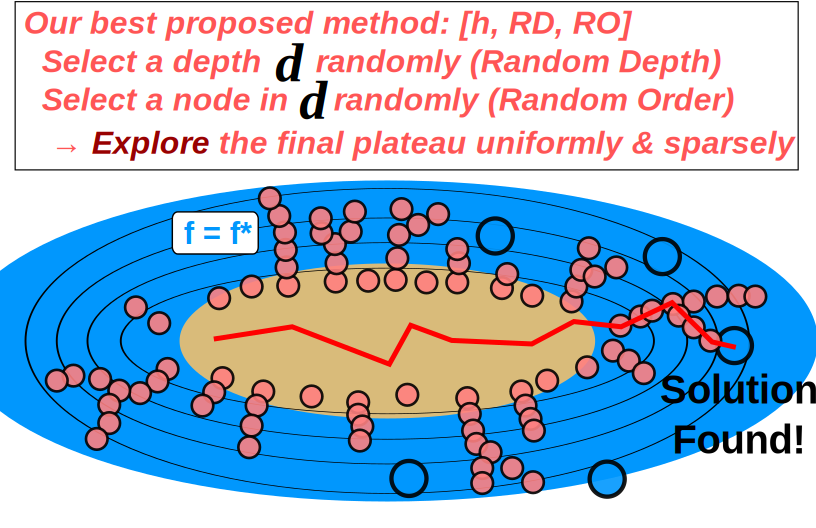
\includegraphics{img/astar/final-plateau7.png}
 \caption{Depth-based diversification allows to search the problem space
 sparsely, avoiding the concentration to particular depths.}
 \label{fig:plateau-depiction-all-optimal}
\end{figure}


We later show that
\fifo and \lifo strategies are incomplete when the size of the plateau
region is inifinite, while our \id is probabilistically complete.

Depth-based tiebreaking has no effect when the target problem contains
positive costs only and the search algorithm uses $h$-based first-level
tiebreaking.  This is because all actions result in an updated
$h$-value, so all nodes have depth 0. In this case, the search is
equivalent to the case of traditional last-resort tiebreaking strategies.

\subsection{Tiebreaking within Depth Buckets}

Since there can be multiple nodes within the same depth bucket,
a last-resort tiebreaking is still necessary to break ties among them.
We could, for example, apply \lifo, \fifo or \ro policies at this level.

\todo{compare id,fifo and id,lifo}

% However we use a Random Order (\ro) policy, which 
% randomly selects an element from the depth bucket selected by the depth-based tiebreaking.
% This is because the effectiveness of the tiebreaking behavior within a bucket
% can be affected by accidental biases, e.g., names/orders of action schema in the PDDL domain
% definition \cite{vallati2015effective}.
% %Finding the best action ordering is not the scope of this paper.
% Thus, we avoid bias at this level of tiebreaking by using \ro and assess its expected/average
% performance.

% Among \fifo, \lifo and \ro, the natural policy is Random Order.
% This is because the effectiveness of the third-level tiebreaking behavior
% is affected by the accidental bias in action ordering in the PDDL domain
% definition.  Recent work \cite{vallati2015effective} showed that the
% planner performance is greatly affected by changing and tuning the action ordering
% (and also variable ordering, but it is irrelevant to the tiebreaking behavior). 
% However, finding the best third-level tiebreaking is not the scope of this paper.
% Thus, focusing on \ro and assess its expected/average
% performance is the most reasonable practice to understand the behavior of second-level,
% depth-based tiebreaking.

